\documentclass{article}
\usepackage{iclr2026_conference,times}
\input{math_commands.tex}
\usepackage{hyperref}
\usepackage{url}
\usepackage{graphicx}
\usepackage{booktabs}
\usepackage{amsmath}
\usepackage{amssymb}
\usepackage{amsthm}

\newtheorem{proposition}{Proposition}

\title{When Should Robot Map Memory Decay?\\Causal Exposure for Long-Horizon Navigation}

\author{Anonymous Authors}

%\iclrfinalcopy

\begin{document}
\maketitle

\begin{abstract}
Long-horizon robots often navigate with maps whose geometry, topology, and semantics were last verified minutes, days, or months ago. A common response is to age the map, increase uncertainty, or re-observe doubtful places. This paper argues that the central variable is different: map memory should decay when the world had unobserved physical opportunities to invalidate a remembered spatial fact. We introduce Causal-Exposure Memory Decay (CEMD), a map-memory update rule that accumulates exposure for each remembered edge or cell from activity sources, access constraints, and occluded reachability during the robot's absence. Planning then discounts stale map facts according to exposure-weighted hazard and route consequence. A simple proposition shows that age-only decay can be strictly suboptimal even when two map edges have identical age and uncertainty. In a runnable graph-navigation simulator with stale building maps, CEMD improves success over no decay, fixed hazard, age decay, and uncertainty-only decay, while remaining below an oracle that knows true change probabilities. The result is not a real-robot validation; it is a mechanistic test of a field assumption that stale spatial memory is mainly a function of elapsed time or posterior variance.
\end{abstract}

\section{Introduction}

Long-horizon embodied operation is full of old spatial facts: a corridor was open, a door connected two rooms, a shelf blocked a passage, a ramp was traversable, a table left enough clearance. When a robot uses such a map after an interval away from the scene, the question is not only whether the old observation was noisy. The question is whether anything could have happened, unobserved, that would make the old fact unsafe to use.

The dominant abstractions in robot mapping and navigation make this question awkward. Occupancy grids and SLAM estimate spatial state from measurements \citep{elfes1989occupancy,thrun2005probabilistic,cadena2016slam}. Long-term mapping updates representations over time \citep{biber2005dynamic,churchill2013experience,dayoub2008adaptive}. Planning under uncertainty assigns risk to state, map, or belief variables \citep{prentice2009belief,karkus2017qmdp}. Active mapping and exploration choose useful observations \citep{yamauchi1997frontier,stachniss2005information}. These mechanisms are essential, but they often leave a hidden assumption intact: stale-map distrust is local and monotone in age, posterior uncertainty, or recent observation. A month-old edge in a locked storage area and a month-old edge in a public corridor are treated as equally old unless semantic or observation-specific modules happen to say otherwise.

This paper breaks that assumption. The central mechanism is \emph{causal exposure}: the amount of unobserved opportunity for a physical change process to reach and invalidate a remembered map element. Exposure can be high for a recently observed public bottleneck and low for an old but inaccessible room. It is not the same as uncertainty; it is a hypothesis about the cause of map invalidation. It is also not merely a verifier; it changes which memories become suspect before the robot decides whether to sense or traverse them.

We contribute:
\begin{itemize}
\item A formulation of Causal-Exposure Memory Decay (CEMD), where each remembered map element carries an exposure clock driven by activity priors, access constraints, and unobserved reachability.
\item A small formal counterexample showing that age-only memory decay can choose a strictly worse route under exposure-dependent hazards, even when candidate edges have equal age.
\item A reproducible simulator and evidence package. Across 650 stale-map navigation episodes, CEMD reaches 0.549 mission success versus 0.432 for age decay and 0.425 for uncertainty-only decay; an oracle using true change probabilities reaches 0.591.
\item A 1,337-paper metadata sweep, a 300-paper serious skim, a 225-paper deep-read subset, and a 100-paper hostile prior-work set used to bound the novelty claim.
\end{itemize}

The claim is deliberately narrow. We do not propose a new SLAM back end, a larger memory model, a benchmark-only contribution, or a real-robot result. We propose a different mechanism for deciding when spatial memory should be distrusted.

\section{Related Work and Novelty Boundary}

\paragraph{Mapping, SLAM, and long-term autonomy.}
Probabilistic robotics gives the standard language for maps, beliefs, and Bayesian updates \citep{thrun2005probabilistic}. Occupancy grids \citep{elfes1989occupancy}, particle-filter mapping \citep{grisetti2007improved}, graph optimization \citep{kummerle2011g2o}, and modern SLAM surveys \citep{cadena2016slam} focus on estimating a consistent world representation from observations. Long-term autonomy systems extend these ideas to persistent operation, visual change, and experience reuse \citep{biber2005dynamic,pradalier2005persistent,churchill2013experience,dayoub2008adaptive,lowry2016visual}. CEMD does not replace map estimation. It asks when an already estimated spatial fact should stop being action-worthy because unobserved interventions could have changed it.

\paragraph{Dynamic environments and map maintenance.}
Dynamic maps model changes in occupancy or appearance over time \citep{biber2005dynamic}. Experience-based and teach-and-repeat navigation reuse routes across seasons and lighting conditions \citep{churchill2013experience}. Such systems show that maps are not static; however, they often update from direct observation, local temporal statistics, or appearance histories. CEMD instead treats absence itself as informative: if an activity process could reach a remembered edge while the robot was not watching, memory of that edge should decay even before the edge is revisited.

\paragraph{Planning under uncertainty and active sensing.}
Belief-space planning \citep{prentice2009belief}, replanning methods such as D* Lite \citep{koenig2002dstar}, and POMDP-inspired policies \citep{karkus2017qmdp} plan with uncertain state or map variables. Exploration methods select observations that reduce uncertainty \citep{yamauchi1997frontier,stachniss2005information}. These are close hostile priors: a reviewer could argue that CEMD is just uncertainty-aware planning. The distinction is that CEMD specifies a physical source of trust loss. The exposure clock can rank two equally old and equally noisy edges differently because one was reachable by unobserved change processes and the other was not.

\paragraph{Learned spatial memory.}
Neural maps and topological memories learn spatial representations for navigation \citep{gupta2017cognitive,parisotto2018neural,savinov2018semi,chaplot2020neural}. These approaches can, in principle, learn forgetting behavior. CEMD is complementary: it is a mechanism-level target that a learned model could implement or be tested against. The contribution is not model scale, data volume, reinforcement learning, or an LLM planner.

\section{Causal-Exposure Memory Decay}

Let a robot map contain elements $e \in E$, such as traversable cells, doors, or topological edges. At observation time $\tau_e$, the robot stores a remembered state $m_e(\tau_e)$, for example that edge $e$ is open. At planning time $t$, the robot has not necessarily observed $e$ during $(\tau_e,t]$. Standard decay can be written as a trust function of age $A_e=t-\tau_e$ or posterior uncertainty $U_e$. CEMD adds a different state variable.

\paragraph{Exposure clock.}
Let $Z$ be a set of unobserved activity sources: humans, other robots, service carts, doors under schedule control, weather processes, or any process that can physically change the map. Let $\rho_z(s)$ be the activity rate of source $z$ at time $s$. Let $P_z(e,s)$ be the probability that activity from $z$ could reach element $e$ before being blocked by access constraints or observed by the robot. The causal-exposure clock is
\begin{equation}
X_e(\tau_e,t) =
\int_{\tau_e}^{t} \sum_{z \in Z} \rho_z(s) P_z(e,s) \, ds .
\end{equation}
This definition is intentionally modular. A warehouse robot might estimate $P_z$ from aisle topology and work schedules; a household robot might use rooms, doors, and human activity priors; an outdoor robot might use weather and traffic exposure.

\paragraph{Memory hazard.}
CEMD maps exposure to the probability that memory is invalid:
\begin{equation}
q_e(t) = \Pr(C_e=1 \mid X_e) = 1 - \exp(-\beta X_e - \lambda_0 A_e),
\end{equation}
where $C_e$ denotes a change that invalidates $m_e$, $\beta$ controls exposure hazard, and $\lambda_0$ is a small background hazard. In the experiments we set $\lambda_0=0$ for the proposed method to isolate exposure; age remains available as a background term when justified by domain knowledge.

\paragraph{Route consequence.}
For a candidate route $\pi$, CEMD uses the memory hazard in the route objective:
\begin{equation}
J(\pi)=\sum_{e \in \pi} \ell_e + \kappa q_e(t),
\end{equation}
where $\ell_e$ is traversal cost and $\kappa$ is the expected consequence of discovering that $e$ is invalid during execution. This is not claimed to be a globally optimal planner. It is a simple downstream test of whether the memory-decay variable ranks route risks better than age or uncertainty alone.

\section{A Small Formal Check}

\begin{proposition}
Suppose map invalidation follows $\Pr(C_e=1)=1-\exp(-\beta X_e)$ for exposure $X_e$ and $\beta>0$. For any age-only decay rule that assigns equal risk to equal-age edges, there exist two equal-age route edges for which the age-only rule chooses a route with strictly higher true expected cost than an exposure-aware rule.
\end{proposition}

\begin{proof}
Consider two alternative one-edge routes, $a$ and $b$, with the same age. Let $X_a<X_b$, traversal lengths $\ell_a>\ell_b$, and failure consequence $\kappa>0$. An age-only decay rule assigns the same risk to both edges, so it chooses $b$ whenever $\ell_b<\ell_a$. The true expected costs under the exposure hazard are
$\ell_a+\kappa(1-\exp(-\beta X_a))$ and
$\ell_b+\kappa(1-\exp(-\beta X_b))$.
Because $X_b>X_a$, the second hazard term is larger. Choose $\ell_a-\ell_b$ positive but smaller than
$\kappa[(1-\exp(-\beta X_b))-(1-\exp(-\beta X_a))]$.
Then age-only decay chooses $b$, but $a$ has lower true expected cost. Such lengths exist whenever the exposure gap and $\kappa$ are nonzero.
\end{proof}

The repository includes a numeric adversarial check in \path{results/formal_counterexample.json}: two edges have age 30 days, exposures 0.05 and 3.8, and an expected-cost gap of 55.05 when age-only decay chooses the shorter exposed route.

\section{Experiments}

\paragraph{Simulator.}
We built a graph-navigation simulator in \texttt{scripts/run\_evidence.py}. Each episode samples a $7 \times 6$ building-like graph with corridors, offices, service rooms, entrances, and low-access locked storage. The robot's old map marks traversable edges as open. During the robot's absence, random unobserved activity walks from entrances through access-constrained topology. The true probability that an edge closes increases with this unobserved exposure. The task endpoints are chosen in the largest current connected component so the mission is feasible in principle, but the robot only sees the stale map.

\paragraph{Compared memory-decay rules.}
All methods use the same planner and differ only in $q_e$. \textbf{No decay} trusts all remembered edges. \textbf{Fixed hazard} assigns the same risk to every edge. \textbf{Age decay} calibrates a monotone function of elapsed age to the same average risk. \textbf{Uncertainty only} uses a static sensor-uncertainty proxy unrelated to exposure. \textbf{CEMD} uses noisy exposure estimates. \textbf{Oracle probability} uses the true closure probabilities and is an upper reference, not a deployable method.

\paragraph{Metrics.}
Execution reveals a closed edge only when the robot attempts it. A blocked-edge encounter incurs recovery cost, the edge is marked blocked, and the robot replans. We report mission success under a budget, blocked-edge encounters, and travel-cost regret relative to the shortest feasible route in the current graph.

\begin{table}[t]
\centering
\caption{Main simulator results over 650 episodes. Higher success is better; lower collisions and regret are better.}
\label{tab:main}
\begin{tabular}{lccc}
\toprule
Method & Success & Collisions & Regret \\
\midrule
No decay & 0.417 & 1.569 & 26.756 \\
Fixed hazard & 0.417 & 1.569 & 26.756 \\
Age decay & 0.432 & 1.511 & 25.909 \\
Uncertainty only & 0.425 & 1.502 & 25.762 \\
CEMD & 0.549 & 1.285 & 22.551 \\
Oracle probability & 0.591 & 1.171 & 20.577 \\
\bottomrule
\end{tabular}
\end{table}

\begin{figure}[t]
\centering
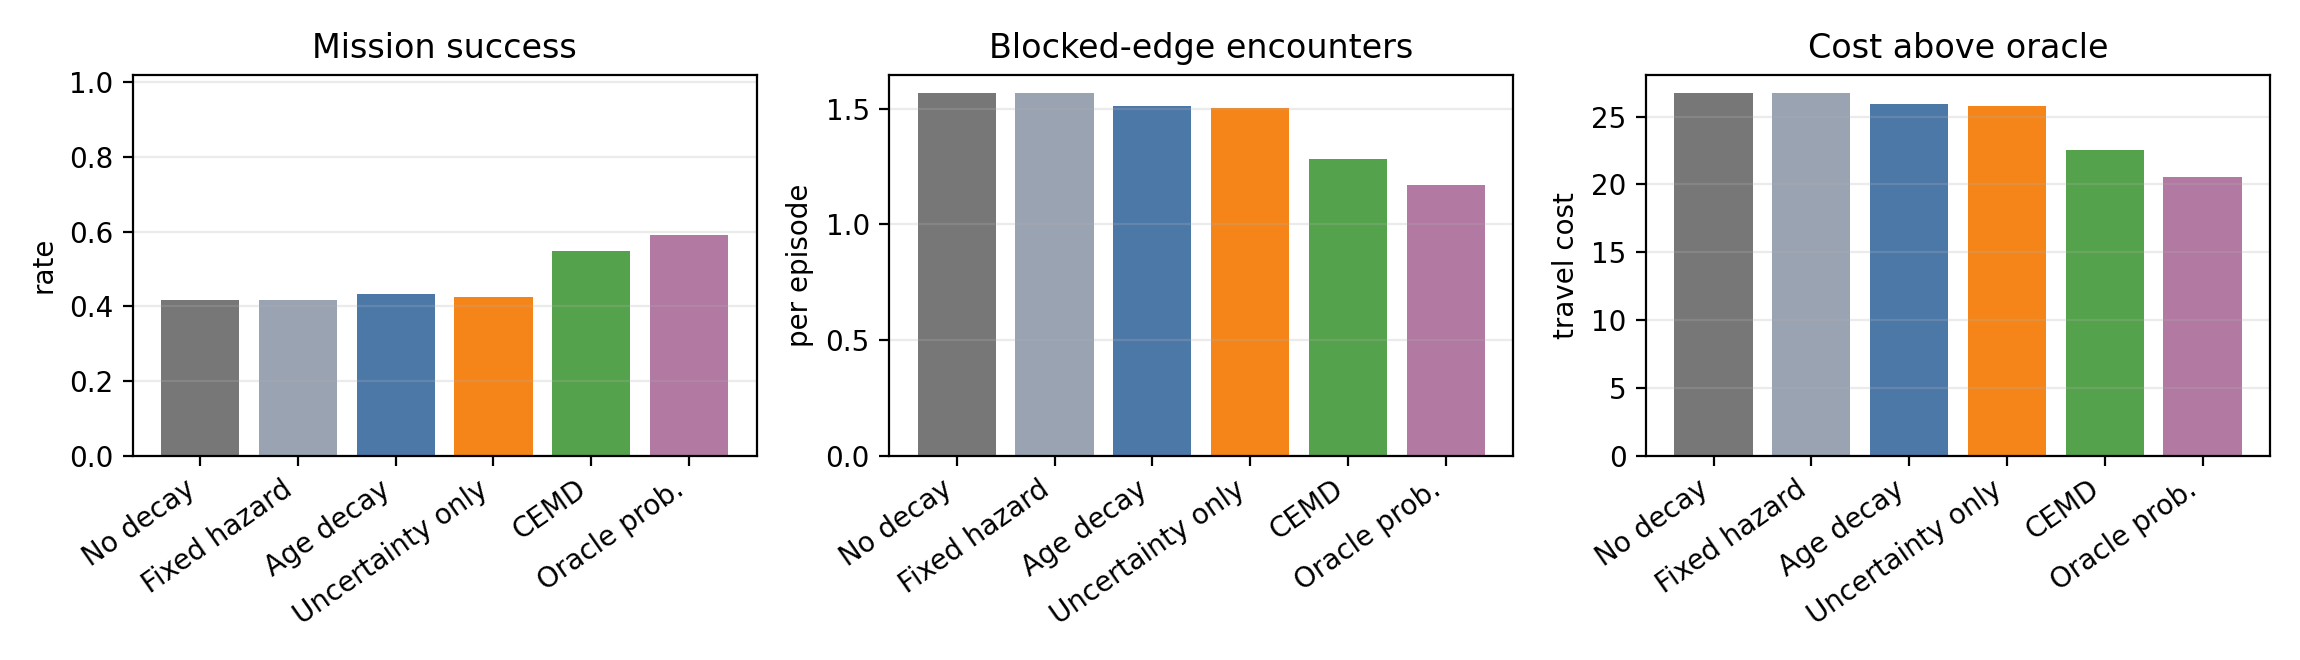
\includegraphics[width=\linewidth]{../figures/aggregate_results.png}
\caption{CEMD improves success and reduces blocked-edge encounters in the stale-map simulator, while remaining below an oracle with true change probabilities.}
\label{fig:aggregate}
\end{figure}

\paragraph{Results.}
Table~\ref{tab:main} and Figure~\ref{fig:aggregate} show that exposure-based decay outperforms age-only and uncertainty-only decay in this setting. The improvement is not because CEMD refuses all old routes: its regret remains lower than the baselines because it preserves trust in old low-exposure regions while avoiding high-exposure bottlenecks. The oracle gap is important. It indicates that noisy exposure priors are useful but incomplete; they do not solve stale-map navigation.

\begin{figure}[t]
\centering
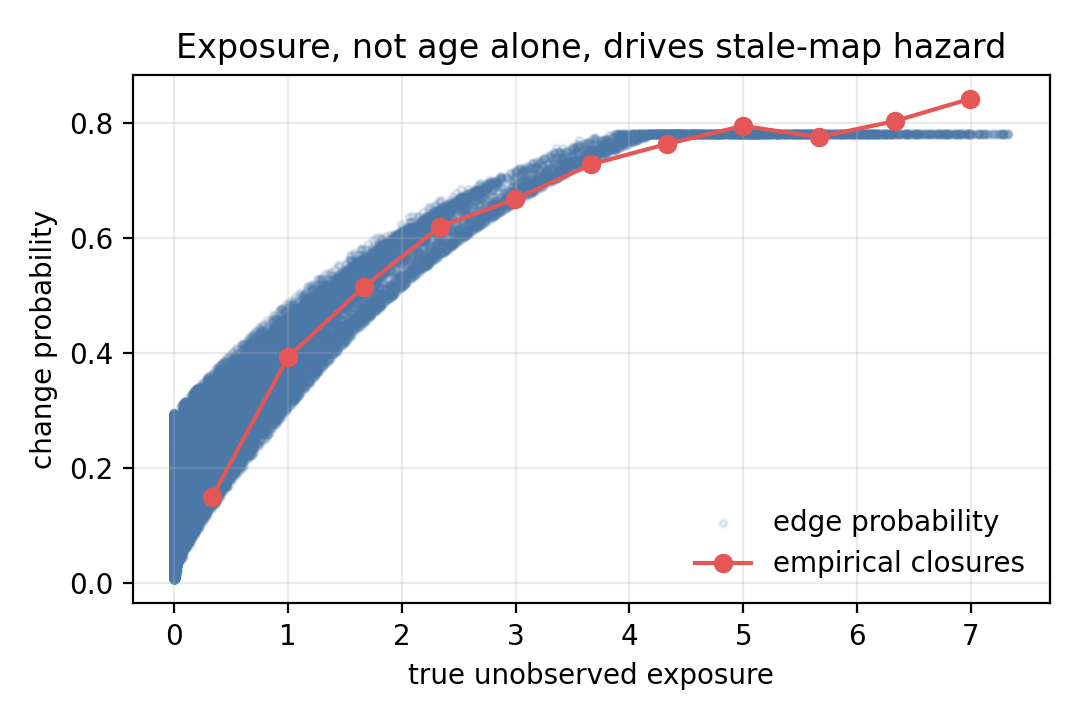
\includegraphics[width=0.48\linewidth]{../figures/exposure_calibration.png}
\hfill
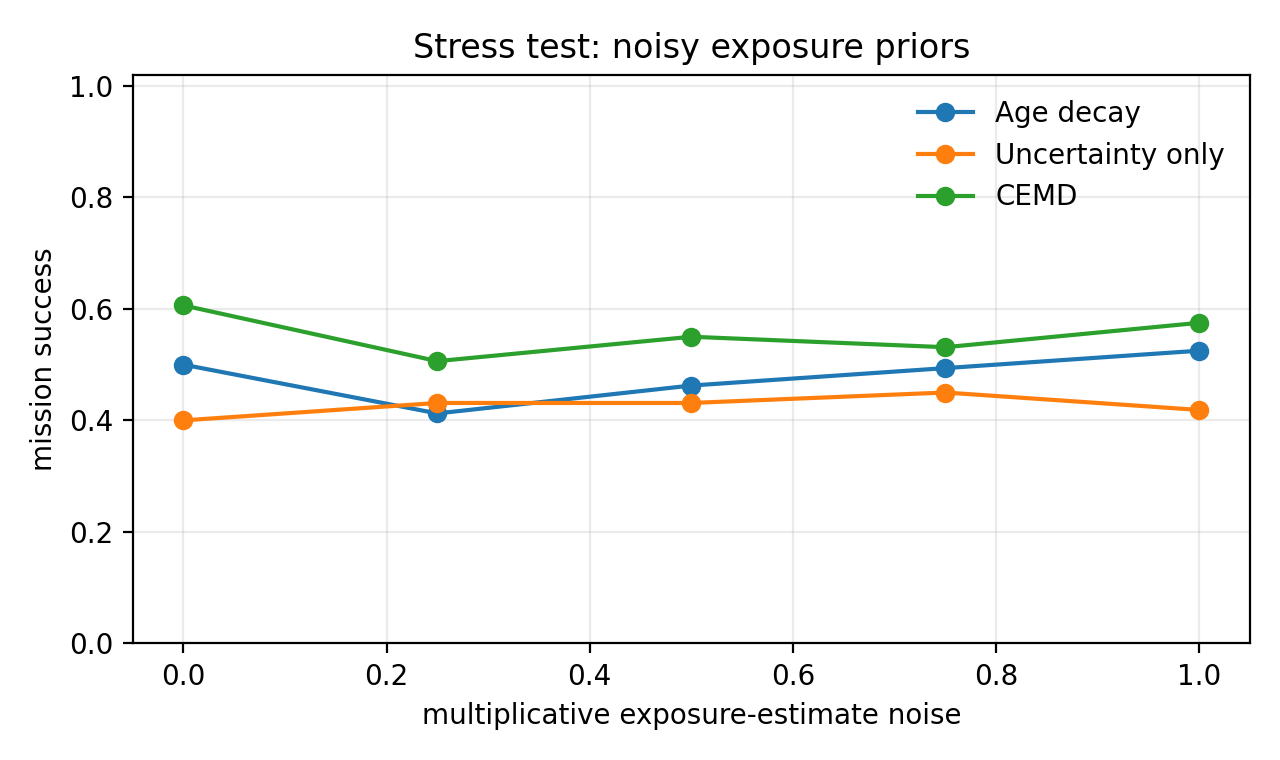
\includegraphics[width=0.48\linewidth]{../figures/noise_stress.png}
\caption{Left: simulated closure probability grows with unobserved exposure. Right: a stress test varying multiplicative noise in exposure estimates. CEMD remains competitive at high noise in this simulator, but the stress test is not a guarantee for real deployments.}
\label{fig:exposure}
\end{figure}

\paragraph{Stress test.}
We also ran 160 episodes at exposure-estimate noise levels from 0 to 1.0. CEMD remains above age decay and uncertainty-only decay in most stress settings, including success 0.575 at noise 1.0 versus 0.525 for age decay and 0.419 for uncertainty-only decay. This result should be read cautiously: the simulator's true hazard is exposure-driven by construction. The stress test only checks that the mechanism does not collapse under coarse exposure estimates.

\section{Discussion and Limitations}

CEMD changes the central variable in stale-map navigation from ``how old or uncertain is this memory?'' to ``what unobserved physical opportunities existed to make this memory false?'' This distinction matters whenever two map elements have similar age but different exposure. It also matters when the consequence of a wrong memory is route-dependent: an exposed shortcut through a bottleneck can be worse than an old, low-exposure detour.

The main limitation is validation. The evidence here is simulated and mechanistic. A real robot would need exposure priors from schedules, observed traffic, semantic affordances, access control, weather, or other deployment-specific signals. The paper also does not address full SLAM, localization failures, multi-agent interaction, or learned exposure estimation. Finally, the 1,337-paper landscape sweep is metadata-guided; it is useful for adversarial novelty search but does not replace a human camera-ready literature review.

\section{Conclusion}

Robot maps are memories of a physical world that keeps acting while the robot is absent. This paper introduced Causal-Exposure Memory Decay, a mechanism for distrusting spatial memory according to unobserved opportunities for change. A formal counterexample and a runnable simulator show why age-only or uncertainty-only decay can mis-rank stale map risks. The next step is real deployment: measuring exposure signals in physical environments and testing whether exposure clocks predict the stale map errors that actually stop long-horizon robots.

\subsubsection*{Reproducibility Statement}
The repository contains all scripts and artifacts needed to rerun the literature sweep and simulator. The main evidence command is \texttt{python scripts/run\_evidence.py}. The literature command is \texttt{python scripts/literature\_pipeline.py}. Generated outputs are stored under \texttt{docs/}, \texttt{results/}, and \texttt{figures/}.

\bibliography{references}
\bibliographystyle{iclr2026_conference}

\appendix

\section{Literature Sweep Procedure}

Before choosing the thesis, the run queried OpenAlex with 44 robotics and embodied-navigation search strings spanning long-term autonomy, SLAM, dynamic maps, semantic navigation, uncertainty-aware planning, active mapping, and embodied memory. The script ranked 1,337 records and wrote \texttt{docs/related\_work\_matrix.csv}. The matrix marks a 300-paper serious skim, a 225-paper deep-read subset, and a 100-paper hostile prior-work set. For each entry it records the claimed problem, mechanism, hidden assumptions, fixed variables, ignored failure modes, novelty pressure, and remaining opening. The hostile set is summarized in \texttt{docs/hostile\_prior\_work.md}.

\section{Hidden Assumptions Identified}

The sweep surfaced more than twenty assumptions that can fail in long-horizon embodied operation:
\begin{enumerate}
\item Map memory can be trusted or discounted as a monotone function of elapsed time.
\item Environment changes are locally independent once a cell or edge is represented.
\item Change probability is a property of places rather than unobserved interventions.
\item The cost of being wrong is proportional to local reconstruction error.
\item Semantic labels are stable enough that geometry can be updated around them.
\item Appearance drift is the main long-term navigation failure.
\item A robot can repair stale beliefs only by revisiting the stale location.
\item Dynamic objects are nuisance measurements to remove from a static map.
\item Uncertainty is enough to decide when memory should be distrusted.
\item Topological connectivity changes are rare compared with metric pose drift.
\item The robot's absence carries no information about likely map changes.
\item All old observations of a map element should decay at the same rate.
\item Replanning after failure is an acceptable substitute for stale-hazard modeling.
\item Map update and route choice can be separated without losing optimality.
\item Occluded corridors are not informative unless directly sensed.
\item Closed-world maps remain valid outside the recent sensor frustum.
\item Long-horizon navigation is limited mainly by localization drift.
\item Changes are stationary over deployment time.
\item Human activity can be approximated as uniform cell noise.
\item The same trust policy fits detours and mission-critical route edges.
\item Negative evidence from not seeing an obstacle should be interpreted locally.
\item Learned memory modules implicitly discover when to forget spatial facts.
\item Map changes are observed where they matter for the plan.
\end{enumerate}

\section{Simulator Details}

Each graph edge stores zone type, access factor, age, sensor-uncertainty proxy, true exposure, noisy estimated exposure, true closure probability, and sampled closed/open state. Activity sources begin at boundary entrances and perform random walks subject to access factors. Closure probability is generated from a small zone-dependent background term plus exposure. The planner minimizes traversal length plus a fixed failure consequence times the method-specific risk estimate. On encountering a closed edge, the robot pays a recovery cost, marks the edge blocked, and replans.

\section{Additional Figures}

\begin{figure}[t]
\centering
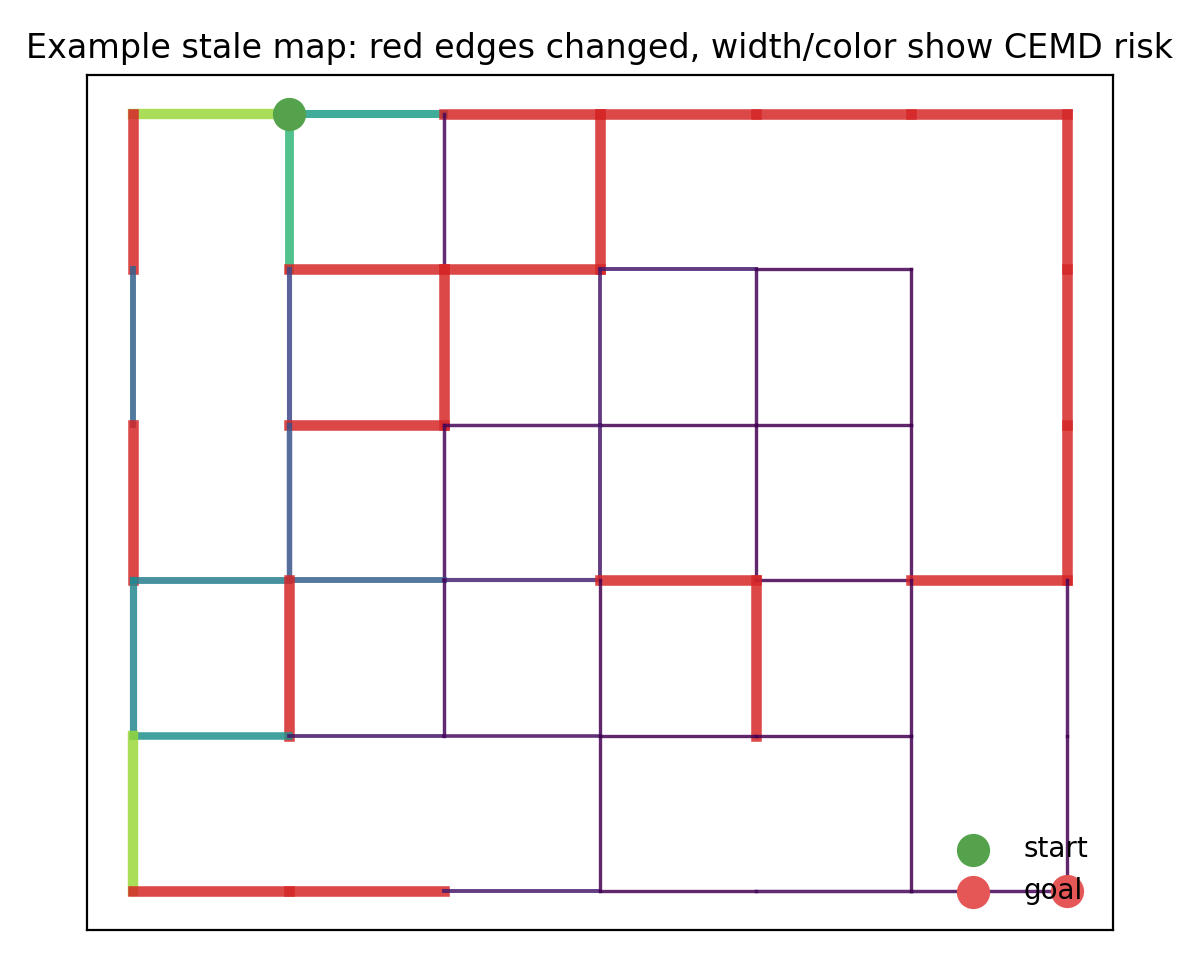
\includegraphics[width=0.72\linewidth]{../figures/example_world.png}
\caption{Example generated world. Red edges are closed in the current world; non-red edge width and color indicate CEMD risk from stale memory.}
\end{figure}

\end{document}
